\chapter{A Credibilidade na Classificação Automática} 
\label{cap::metodo}

Como mostrado no Capítulo~\ref{cap::related}, o termo credibilidade já foi utilizado com diferentes significados na literatura. Nesse trabalho, estudamos especificamente com o conceito de credibilidade no contexto de classificação automática. Definimos que classificar automaticamente é estipular a qual classe um exemplo pertence através do uso de algoritmos, sem auxílio humano, partindo da premissa que quaisquer dois exemplos de uma mesma classe apresentam um valor semântico próximo.   
%linkar isso com credibilidade .... Assumimos que a credibilidade de uma entidade reflete o quanto ela agrega a uma tarefa sendo executada.

Sendo assim, a credibilidade explora o conhecimento da classe dos exemplos de treino e tenta aproximar aqueles que são mais significativos para o exemplo de teste.
Logo, a semântica contida nos exemplos de treino e teste, seja por meio de seus atributos ou relacionamentos, é capturada pelo calculo da credibilidade.
Dessa forma, a credibilidade de um exemplo é diretamente proporcional ao quanto que aquele exemplo ajuda na discriminação das diferentes classes existentes.
Isso significa que um exemplo $e_{1}$ tem um valor de credibilidade maior que outro exemplo $e_{2}$, caso ele forneça maiores indícios para descobrirmos a qual classe um terceiro exemplo $e_{3}$ pertence. 

Definimos a credibilidade de um exemplo como um número real que incorpora diversos fatores quantitativos em um único valor dentro de uma faixa predefinida, chamada de escala de credibilidade. Temos também que quanto maior é esse valor, mais importante é esse exemplo para ajudar na tarefa de classificação. Mesmo considerando somente a classificação automática, esses fatores variam de acordo com a aplicação. Por exemplo, no contexto de classificação de documentos, podemos considerar os termos, os autores, as citações, os meios de vinculação ou mesmo o ano de lançamento de um documento como fatores a serem modelados pelo que denominamos ``funções de credibilidade'', que em geral relacionam um desses fatores e cada uma das possíveis classes em um número real, $\mathbb{F} \times \mathbb{C} \mapsto \mathbb{R}^+$. 

%Nesse capítulo, explicaremos dois classificadores automáticos muito utilizados, \textsc{KNN} e \textit{Naïve Bayes} e depois iremos mostrar como incorporamos as funções de credibilidade da forma mais geral possível.

%--> TODO: realocar--->>> O valor da credibilidade apresenta um comportamento assintótico crescente e monotônico, ou seja, ao calcularmos a credibilidade de uma entidade levando em conta todos os possíveis fatores produziremos um valor mais significativo de credibilidade do que quando calculamos levando em conta apenas um subconjunto desses fatores.

Já existem algumas métricas que podem ser usadas como funções de credibilidade, como a distância média utilizada pelo algoritmo dos $K$ vizinhos mais próximos (\textsc{KNN}). Nela, quanto maior é a distância do exemplo de teste para os exemplos de treinamento, menor é a credibilidade da informação provida. Podemos ainda considerar algumas métricas que levam em conta o valor discriminativo dos atributos de um exemplo, como as métricas \textsc{TD-IDF} e \textit{dominância}, boas estimadoras de credibilidade. Ambas serão explicadas com maiores detalhes na Seção~\ref{sec::pg_cred_baseada_conteudo}, entretanto, por enquanto, podemos dizer que a primeira provê um medida global de significância para um atributo, enquanto, a segunda provê um valor local. 
%Uma boa ideia seria unir os benefícios providos por ambas, porém como realizar essa junção é um desafio. Uma abordagem simples é realizar uma soma de pesos provenientes de cada uma das métricas, porém essa pode ser uma abordagem muito simplista que não considera nenhuma correlação entre as métricas.

%versao com NB + KNN
Finalmente, uma vez definido um valor para a credibilidade, temos que incorporá-lo aos algorítimos de classificação. Isso quer dizer que, no contexto de classificação automática, os algoritmos devem ser alterados de forma a levar em consideração o valor da credibilidade dos exemplos utilizados. Nesse capítulo, explicamos e mostramos como incorporamos a credibilidade em dois algoritmos clássicos, o \textit{Naïve Bayes} e o algoritmo dos $K$ vizinhos mais próximos, \textsc{KNN}. O principal motivo para utilizarmos o \textit{Naïve Bayes} é que esse apresenta um bom desempenho  para classificação de documentos (\cite{salles10}), que é o principal tipo de classificação que tratamos nesse trabalho. Embora o algoritmo \textit{Support Vector Machine} (\textsc{SVM}) possa superar o \textit{Naïve Bayes} em alguns cenários de classificação de documentos, o custo computacional de utilizar o \textsc{SVM} em um problema de classificação multi-classe é um obstáculo a ser levado em conta. Baseado no compromisso entre o custo computacional e os resultados obtidos, decidimos por utilizar o algoritmo \textit{Naïve Bayes}, detalhado na Seção~\ref{subsec::cred_nb}. Queremos também mostrar que a credibilidade não está atrelada a apenas um classificador e, portanto, também realizamos modificações no \textsc{KNN}. Escolhemos o \textsc{KNN}, explicado na Seção~\ref{subsec::cred_knn}, por sua simplicidade, apresentando apenas um parâmetro, seus bons resultados em bases de bio-informática (citar) e por advogarmos que o \textsc{KNN} já utiliza uma credibilidade básica em sua própria estrutura. Finalmente, as Seções~\ref{subsubsec::nb_cred} e \ref{subsubsec::knn_cred} abordam como podemos incorporar as funções de credibilidade nos algoritmos \textit{Naïve Bayes} e \textsc{KNN}, respectivamente.

%%%%%%%%%%%%%%%%%%%%------------------------------------------------------------------------------------------------------------------------------------%%%%%%%%%%%%%%%%%%%%%%%%%%%%%%%%%
%%%%%%%%%%%%%%%%%%%%------------------------------------------------------------------------------------------------------------------------------------%%%%%%%%%%%%%%%%%%%%%%%%%%%%%%%%%
%%%%%%%%%%%%%%%%%%%%------------------------------------------------------------------------------------------------------------------------------------%%%%%%%%%%%%%%%%%%%%%%%%%%%%%%%%%

\section{Classificador \textit{Naïve Bayes}.}
\label{subsec::cred_nb}

Nessa seção, explicamos o funcionamento do algoritmo \textit{Naïve Bayes} original. É importante termos em mente a versão original do mesmo para que possamos compará-la à versão na qual a credibilidade é incorporada (ver Seção~\ref{subsubsec::nb_cred}). Referências mais detalhadas do \textit{Naïve Bayes} podem ser encontradas em \cite{DHS01} e \cite{Manning08}.

De uma maneira sucinta, porém prática, podemos utilizar os seguintes passos para definir o classificador \textit{Naïve Bayes}:

\begin{enumerate}
    \item Cada um dos exemplos do conjunto de treinamento pode ser visto como uma tupla $D$-dimensional, $X$ = ($x_1$, $x_2$, $x_3$, ..., $x_D$), onde $x_i$ é o valor referente ao atributo $A_i$ no exemplo $X$. É importante ressaltar que para um atributo $A_i$, podemos ter valores distintos de $x_i$ nos vários exemplos de treino. Tipicamente, em um problema de classificação com atributos numéricos, o atributo $x_i$ pode assumir qualquer valor real. Já em um problema de classificação categórico, $x_i$ pode assumir uma faixa controlada de valores discretos. Em classificação de documentos, por exemplo, $x_i$ pode ser qualquer valor inteiro natural, representando o número de vezes que temos um termo $A_i$ em $X$. Vale a pena lembrar também que podemos ter a coexistência de atributos numéricos e categóricos em uma mesma base de dados.
    

    \item Suponha que existem \textit{M} classes, $c_1$, $c_2$, ..., $c_\textit{M}$, formando o conjunto de possíveis classes $\mathbb{C}$. Dado um determinado exemplo $X$, o classificador Bayesiano prevê que $X$ pertence à classe que tiver a maior probabilidade a \textit{posteriori} $P(c_j|X)$. Ou seja, o classificador \textit{Naïve Bayes} diz que $X$ pertence a $c_j$, se e somente se:
        
\begin{equation}\label{eqn::max_pcgivenx}
   P(c_{j}|X) > P(c_{k}|X) \;\;\;\;\;\forall k,\; 1 \le k \le M, \; k \not= j,
\end{equation}
onde $P(A|B)$ é um valor real entre 0.0 e 1.0 que define a probabilidade do evento A ser verdadeiro, dado que o evento B ocorreu. No caso, podemos interpretar a expressão $P(c_j|X)$ como a probabilidade da classe correta ser $c_j$ dado o exemplo $D$-dimensional $X$ = ($x_1$, $x_2$, ..., $x_D$).

    \item Necessitamos, portanto, de uma forma de calcular a probabilidade a \textit{posteriori} $P(c_j| X)$, que pode ser definida pelo teorema de Bayes como:
\begin{equation}\label{eqn::bayes}
   P(c_{j}|X) = \frac{P(X|c_j) \times P(c_j) }{P(X)}
\end{equation}

    \item Da Equação~\ref{eqn::bayes} temos que $P(c_j)$ pode ser obtida simplesmente calculando a proporção de exemplos da classe $c_j$ que temos em nosso conjunto de treinamento. Além disso, a probabilidade $P(X)$ é uma constante independente da classe e, por isso, não precisamos calculá-la.
       
    \item Obter $P(X|c_j)$ é uma tarefa extremamente cara computacionalmente. Porém podemos utilizar a premissa ``ingênua'' \footnote{O nome do algoritmo Naïve Bayes provém dessa premissa simplificadora.} de que os valores dos atributos de um exemplo $X$ são condicionalmente independentes um dos outros, dada uma certa classe. Logo,

\begin{equation}\label{eqn::classindependence}
   P(X|c_{j}) = \prod^{n}_{i=1}{P(x_i|c_j) }
\end{equation}

\item O valor de cada termo $P(x_i|c_j)$ da Equação~\ref{eqn::classindependence} é usualmente calculado de forma diferente caso o atributo $A_i$ seja categórico, textual ou numérico. A seguir mostramos as formas mais comuns vistas na literatura:
    \begin{itemize}

        \item Caso $A_i$ seja categórico, então $P(x_i|c_j)$ é o número de exemplos no treinamento que pertencem a classe $c_j$, nos quais o valor de $A_i$ é $x_i$, dividido pelo número de exemplos da classe $c_j$ no treino:

    \begin{equation}\label{eqn::nbcattexto}
        P(x_i|c_j) = \frac{ F_{x_{i}c_{j}} }{ F_{c_{j}} },
    \end{equation}
        onde $F_{x_{i}c_{j}}$ é o número de vezes que temos o termo $x_i$ nos exemplos de treino da classe $c_j$ e $F_{c_{j}}$ é o número de exemplos de treino da classe $c_j$.
        
        \item Caso $A_i$ seja textual, temos uma versão ligeiramente diferente que pode ser expressa na seguinte fórmula:

    \begin{equation}\label{eqn::nbcattexto}
        P(t_i|c_j) = \frac{ F_{t_{i}c_{j}} }{ \sum\limits^{D}_{k = 1} { } F_{t_{k}c_{j}} },
    \end{equation}
        onde $F_{t_{i}c_{j}}$ é o número de vezes que temos o termo $t_i$ nos exemplos de treino (aqui, documentos de treino) da classe $c_j$ e $D$ é o número de atributos existentes (tamanho do vocabulário conhecido).

        \item Caso $A_i$ seja um atributo numérico, tipicamente um valor real, então assumimos que o valor $x_i$ do atributo $A_i$ é dado por uma distribuição Gaussiana de média $\mu_i$ e desvio padrão $\sigma_i$ e podemos usar a seguinte fórmula para calcular $P(x_i|c_j)$:
    \begin{eqnarray}\label{eqn::nbnumerico}
        P(x_i|c_j) & = & g(x_i, \mu_{ic_j}, \sigma_{ic_j})  \\
        g(x, \mu, \sigma) & = & \frac {1} { \sqrt{2\pi\sigma} } e^{ -\frac{(x-\mu)^2}{2\sigma^2}  } 
    \end{eqnarray}
        onde $\mu_{ic_j}$ e $\sigma_{ic_j}$ são a média e o desvio padrão dos valores de $A_i$ nas tuplas de treinamento da classe $c_j$. 

    \end{itemize}

    \item Finalmente, podemos juntar as Equações \ref{eqn::max_pcgivenx} e \ref{eqn::classindependence}, definindo:

    \begin{equation}\label{eqn::nbfinal}
    \textit{Classe Atribuída} = \arg\max_{c_j \in \mathbb{C}}P(X|c_j) = \frac{F_{c_j}}{N} \cdot {\prod^{D}_{i=1}{P(x_i|c_j) }},
    \end{equation}
    onde $\mathbb{C}$ é o conjunto das possíveis classes, $N$ é o número de exemplos no conjunto de treinamento, $F_{c_j}$ é o número de exemplos da classe $c_j$ em $N$ e $D$ é o número de atributos existentes.


\end{enumerate}

%%%%%%%%%%%%%%%%%%%%------------------------------------------------------------------------------------------------------------------------------------%%%%%%%%%%%%%%%%%%%%%%%%%%%%%%%%%

\section{Incorporando a Credibilidade no \textit{Naïve Bayes}.}
\label{subsubsec::nb_cred}

Dada a formulação descrita na Seção~\ref{subsec::cred_nb}, aqui explicamos como o \textit{Naïve Bayes} pode ser modificado para incorporar o conceito de credibilidade. Primeiramente, modelamos a credibilidade de um exemplo inspirado unicamente em seus atributos, assim como mostrado na Seção \ref{subsubsec::nbcredatributos}. Por sua vez, na Seção \ref{subsubsec::nbcredgrafos}, mostramos como tratar a credibilidade em um nível mais alto, tentando tirar proveito das relações existentes entre as instâncias de treinamento e a instância de teste, a princípio, sem nos preocuparmos com seus atributos.

\subsection{\textit{Naïve Bayes} com Credibilidade Baseada nos Atributos.}
\label{subsubsec::nbcredatributos}

A credibilidade de uma instância $X$, baseada no seus atributos, procura determinar para cada atributo $A_i = x_i$ em $X$, o quanto $x_i$ contribui para conseguirmos prever a qual classe $X$ pertence. De maneira geral, calculamos a credibilidade de $x_i$, referente ao atributo $A_i$ em relação a classe $c_j$, como uma função $Cr_{cont}(x_i, c_j)$ e podemos facilmente acoplá-la a Equação~\ref{eqn::classindependence}, resultando em:

\begin{equation}\label{eqn::classindependence_conteudo}
   P(X|c_{j}) = \prod^{D}_{i=1}{(P(x_i|c_j) \cdot Cr_{cont}(x_i,c_j))} 
\end{equation}

Dessa forma, avaliamos para cada atributo $A_i$ o quanto ganhamos sabendo que $A_i$ tem o valor de $x_i$, dada cada uma das classes $c_j$. Existem várias métricas conhecidas na literatura que podem ser utilizadas para medirmos a influência de um termo na determinação da classe de uma instância de teste, como o \textit{Ganho de informação} (\textsc{IG} - do inglês \textit{Information Gain}) e a \textit{Medida de Ambiguidade} (\textsc{AM} - do inglês \textit{Ambiguity Measure}). Ambas, como veremos, poderiam vir a ser boas funções de credibilidade. 


    Com um pouco mais de detalhe, a \textit{Medida da Ambiguidade} definida em \cite{Mengle08} procura verificar a importância do valor de atributo baseado no número de vezes que aquele valor aparece conjuntamente com uma determinada classe. Matematicamente, temos:
\begin{equation}\label{eqn::classindependence_conteudo_am}
   Cr_{cont} = AM(x_i, c_j) = \frac{ F_{x_{i}c_{j}}}{\sum\limits_{c_k \in \mathbb{C}} F_{x_{i}c_{k}}},
\end{equation}
   onde $F_{x_{i}c_{j}}$ é o número de instâncias no treino com $A_i$ valendo $x_i$ e pertencentes a classe $c_j$. Especificamente, no problema de classificação de documentos, modelamos como \textsc{AM} usando $F_{t_{i}c_{j}}$ que é a frequência do termo $t_i$ referente ao atributo $A_i$ nos documentos de classe $c_j$.

    Por sua vez, o \textit{Ganho de Informação} (ver \cite{forman03}) mede o quanto de informação adquirimos para prever uma classe, sabendo o valor de um certo atributo. Formalmente, temos:
\begin{equation}\label{eqn::classindependence_conteudo_ig}
   Cr_{cont} = IG(x_i, c_j) = \sum_{c \in \{c_j, \overline{c_j}\}}\sum_{t \in \{x_i, \overline{x_i}\}}P(t|c) \cdot \log_2\frac{P(t|c)}{P(t) \cdot P(c)}.
\end{equation}

    Porém não sabemos qual das duas métricas funciona melhor como uma função de credibilidade, pois isso é uma tarefa dependente da aplicação. Além disso, podemos combiná-las para conseguirmos uma função que venha a obter ainda melhores resultados. Na verdade, existem muitas outras métricas que podemos utilizar como função de credibilidade baseada nos atributos. Listamos e explicamos cada uma das métricas que foram utilizadas nesse trabalho na Seção~\ref{subsec::pg_metricas_conteudo}. 
É importante destacar que, devido ao grande número de métricas, testar cada uma das suas possíveis combinações é uma tarefa combinatória muito cara computacionalmente, e, portanto, inviável. Por esse motivo, empregamos a \textit{Programação Genética} (\textsc{PG}), um mecanismo capaz de combiná-las de forma elegante, formando funções de credibilidade mais robustas. Dedicamos o Capítulo~\ref{cap::programacao_genetica} exclusivamente para abordamos em detalhes como usamos \textsc{PG} na geração de funções.

%%%%%%%%%%%%%%%%%%%%------------------------------------------------------------------------------------------------------------------------------------%%%%%%%%%%%%%%%%%%%%%%%%%%%%%%%%%

\subsection{\textit{Naïve Bayes} com Credibilidade Baseada em Relacionamentos.}
\label{subsubsec::nbcredgrafos}

A credibilidade da pertinência de um exemplo a uma classe também pode ser mensurada baseando-se nos relacionamentos existentes entre o exemplo e o conjunto de treinamento. Anteriormente, estimamos o quanto o conhecimento de que um atributo $A_i$ tem valor $x_i$ nos ajuda a classificar um exemplo em relação a uma classe $c_j$. Dessa vez, queremos calcular o quanto ganhamos explorando os relacionamentos existentes entre o exemplo de teste e os exemplos de treinamento. Para tanto, necessitamos que um relacionamento possa ser estabelecido entre os exemplos da base de treinamento e teste. Alguns relacionamentos comuns na tarefa de classificação de documentos, por exemplo, são autoria e citação. No primeiro, criamos um elo entre dois documentos se eles têm um mesmo autor em comum e, no segundo, criamos um elo entre eles se um cita ou é citado pelo outro. Temos relacionamentos bastante parecidos em uma base de músicas ou vídeos, nos quais músicas (filmes) de mesmo gênero ou mesmo cantor (ator ou diretor) estariam relacionadas. É oportuno destacar que podemos tratar todos esses relacionamentos como um grafo.

Formalmente, um grafo $G = (V,E)$ é uma estrutura composta por um conjunto $V$ de vértices e outro $E$ de arestas. Os vértices representam os exemplos do conjunto de treinamento os quais estamos interessados, sejam documentos, músicas ou enzimas. As arestas, por sua vez, cumprem o papel de relacionar os exemplos segundo algum critério. Por exemplo, podemos modelar um grafo de autoria, definindo uma aresta $e(d_1,d_2)$ se $d_1$ e $d_2$ têm autores em comum. Podemos ir mais além e atribuir um valor inteiro $k$ para essa aresta, significando que $d_1$ tem $k$ autores em comum com o documento $d_2$.

De forma geral, dado um relacionamento entre os exemplos, é possível construir um grafo utilizando todo o conjunto de treinamento. Entretanto, como estamos interessados em avaliar como os relacionamentos dentro de uma mesma classe podem nos ajudar a prever a qual classe pertence o exemplo de teste avaliado, decidimos por montar um grafo para cada possível classe. Ou seja, tomamos todos os exemplos de treinamento da classe $c_i$ e construímos o grafo $G_i$. Assim podemos analisar com maior clareza o relacionamento do teste com cada grafo de cada classe, evitando interferências de relações entre exemplos de treino de classes diferentes. Destacamos que é esperado que o exemplo de teste se conecte a mais de um grafos, representando seus vários relacionamentos com classes distintas contidas no treino.

Na Figura~\ref{fig::grafo}, temos uma exemplificação dessa situação. Nela, o exemplo de teste é representado por um triângulo e contém arestas para todos os exemplos da classe Quadrado e uma aresta para um indivíduo da classe Círculo. O que apresenta indícios para acreditarmos que o triângulo não pertence a classe Quadrado. Dependendo da função que utilizarmos para a credibilidade, a classe dos círculos ou dos losangos pode se tornar mais ou menos importante, porém temos certo que a credibilidade da classe Quadrado, baseando no relacionamento modelado, é muito baixa ou nula.

\begin{figure}[ht!]
\centering
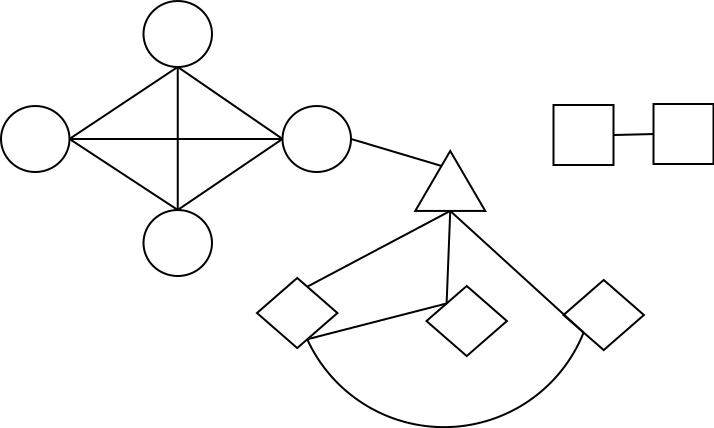
\includegraphics[width=0.7\textwidth]{figures/grafo.png}
\caption{A instância de teste triângulo está ligada ao grafo formado pela classe dos círculos e dos losangos, porém não apresenta ligações com os quadrados.}
\label{fig::grafo}
\end{figure}

Para cada grafo representando uma classe, podemos calcular a credibilidade do exemplo de teste para aquela classe e a incorporar ao classificador Bayesiano. Decidimos modificar a Equação~\ref{eqn::classindependence}, sugerindo a seguinte fórmula:

\begin{equation}\label{eqn::nbcredgrafo}
P(X|c_{j}) = \prod^{D}_{i=1}{(P(x_i|c_j)) \cdot (\alpha + Cr_{rel}(X,c_j)) } 
\end{equation}

Como na Equação~\ref{eqn::classindependence}, continuamos calculando o produtório dos atributos que compõem o exemplo $X$, porém calculamos também a credibilidade de $X$ em relação a classe $c_i$. Utilizamos um fator $\alpha$ para evitarmos que a falta de uma aresta entre $X$ e instâncias da classe $i$ possa resultar em uma probabilidade nula de que $X$ seja da classe $i$. Note que podemos, sem problema algum, juntar as Equações \ref{eqn::classindependence_conteudo} e \ref{eqn::nbcredgrafo} dando origem a um classificador Bayesiano que leva em conta tanto a credibilidade dos atributos quanto a dos relacionamentos:

\begin{equation}\label{eqn::nbcredcompleta}
P(X|c_{j}) = \prod^{D}_{i=1}{(P(x_i|c_j) \cdot Cr_{cont}(x_i,c_j)) \cdot (\alpha + Cr_{rel}(X,c_j)) } 
\end{equation}

%TODO: citacao faltando
Pelo fato de modelarmos os relacionamentos existentes entre os exemplos por meio de grafos, decidimos por utilizarmos as diversas métricas de redes complexas [cite], a fim de explorarmos as propriedades dos grafos criados. Um exemplo simples de uma dessas métricas é contar o número de vizinhos de um vértice, $viz(v,c_j)$. Essa função retornaria o número de conexões o vértice $v$ tem com seus vizinhos que são da classe $c_j$. Partimos do pressuposto que se um vértice for importante para uma determinada classe $j$, $viz(v,c_j)$, será um valor superior para aquela classe. Na Figura~\ref{fig::grafo}, a classe losango seria a de maior credibilidade para classificarmos o triângulo, baseando nessa métrica. Outras várias métricas importantes podem ser listadas e combinada, sendo assim, atribuímos toda a Seção~\ref{sec::pg_cred_baseada_grafos} para maiores detalhes.  


%%%%%%%%%%%%%%%%%%%%------------------------------------------------------------------------------------------------------------------------------------%%%%%%%%%%%%%%%%%%%%%%%%%%%%%%%%%
%%%%%%%%%%%%%%%%%%%%------------------------------------------------------------------------------------------------------------------------------------%%%%%%%%%%%%%%%%%%%%%%%%%%%%%%%%%
%%%%%%%%%%%%%%%%%%%%------------------------------------------------------------------------------------------------------------------------------------%%%%%%%%%%%%%%%%%%%%%%%%%%%%%%%%%
%%%%%%%%%%%%%%%%%%%%------------------------------------------------------------------------------------------------------------------------------------%%%%%%%%%%%%%%%%%%%%%%%%%%%%%%%%%

\section{Classificador \textsc{KNN}.}
\label{subsec::cred_knn}

%No decorrer dessa seção, explicaremos o algoritmo dos K vizinhos mais próximos (do inglês, \textit{K-Nearest Neighbor}, KNN). Da mesma forma que fizemos com o \textit{Naïve Bayes}, dedicamos uma seção, Seção~\ref{subsubsec::knn_cred}, exclusivamente para abordarmos o \textsc{KNN} integrado a credibilidade. 

O algoritmo dos $K$ vizinhos mais próximos (\textsc{KNN}) é conhecido por ser um método de aprendizado baseado em analogias, ou seja, comparamos o teste com os exemplos contidos no treinamento a fim de conseguirmos encontrar aqueles com maior semelhança. 
Tipicamente, cada exemplo existente é uma tupla de $D$ dimensões e representa um ponto em um espaço $D$-dimensional. 
Quando um novo exemplo de teste, de classe desconhecida, necessita ser classificado, o algoritmo \textsc{KNN} procura nesse espaço $D$ dimensional pelos $k$ exemplos do treinamento que estão mais perto do teste. 
Por fim, os $k$ vizinhos mais próximos realizam uma votação para escolherem qual será a classe que o teste pertence.

Na Figura~\ref{fig::knn}, temos um triângulo que representa o exemplo de teste, os quadrados e losangos, representando os exemplos de treinamento pertencentes a classe Quadrado e Losango, respectivamente. As orbitas circulares existentes na figura são epicêntricas e servem apenas para fins didáticos.
Por essa figura, vemos a importância do parâmetro $k$ na decisão da classe que um objeto pertence. Considerando que cada objeto tem o mesmo peso na votação, caso $k=1$, escolhemos a classe bola para o exemplo de teste, entretanto, se $k=5$, escolhemos a classe Quadrado. Para valores de $k$ entre 2 e 4, como temos 3 vizinhos a uma mesma distância, necessitamos de algum método de desempate. Em nosso trabalho, ordenamos os vizinhos primeiramente pela distância até o teste e depois por um identificador único. Dessa forma, minimizamos problemas relativos a ordem como os exemplos de treinamento são apresentados.

\begin{figure}[ht!]
\centering
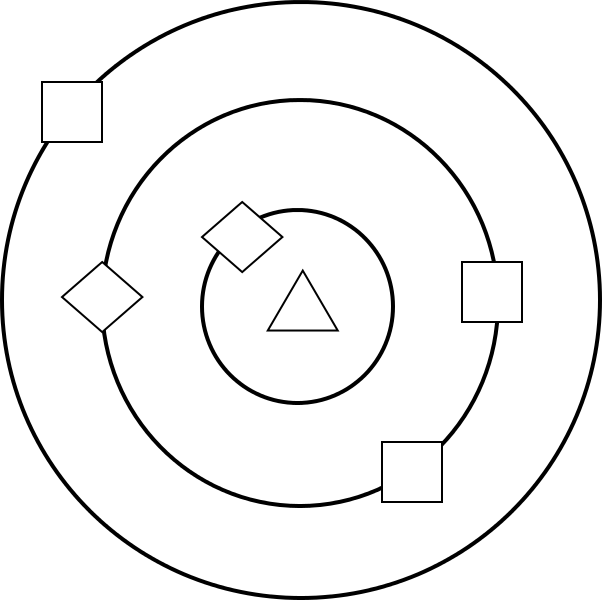
\includegraphics[width=0.5\textwidth]{figures/knn.png}
\caption{O algoritmo dos $k$ vizinhos mais próximos.}
\label{fig::knn}
\end{figure}

Como vimos, uma parte fundamental do \textsc{KNN} é podermos calcular o quão próximo uma instância de teste está das instâncias de treinamento. 
Essa proximidade é tipicamente calculada por uma métrica de distância que pode variar de problema para problema. Utilizamos 3 métricas diferentes, dependendo se estamos classificando um atributo $A_i$ que seja categórico, numérico ou textual. Para duas instâncias $X_1 =  (x_{11}, x_{21}, x_{31}, ..., x_{D1})$ e $X_2 = (x_{12}, x_{22}, x_{32}, ..., x_{D2})$, nas quais $x_{ij}$ representa o valor do atributo $A_i$ para a instância $j$, temos que, caso $A_i$ seja:

\begin{itemize}

\item numérico, utilizamos a distância Euclidiana:

\begin{equation}\label{eqn::distancia_euclidiana}
    dist(X_1, X_2) =  \sqrt{\sum_{i=1}^D (x_{i1}-x_{i2})^2}
\end{equation}

    Com o intuito de evitar que um atributo com grande escala de valores sobreponha um outro atributo de uma menor escala, empregamos a normalização \textit{min-max} para todos os valores $x_i$ do correspondente atributo $A_i$: 

\begin{equation}\label{eqn::distancia_euclidiana}
    x'_{i} =  \frac{x_{i} - min_{A_i}}{ max_{A_i} - min_{A_i} }
\end{equation}

\item categórico, comparamos $X_1$ e $X_2$ e somamos uma unidade a distância entre as instâncias para cada $x_i$ que tenha valores distintos entre $X_1$ e $X_2$.

\begin{equation}\label{eqn::distancia_cat}
   dist(X_1, X_2) = \sum_{1 < i < D \ \wedge \ x_{i1} \neq x_{i2}} 1.0
\end{equation}

\item textual, tomamos a distância dos cossenos entre os dois exemplos $X_1$ e $X_2$ e invertemos o seu sinal. Ou seja, sendo $||X_j|| = \sqrt{ (x_{1j} \cdot w_{1j})^2 + (x_{2j} \cdot w_{2j})^2 + (x_{3j} \cdot w_{3j})^2 + ... + (x_{Dj} \cdot w_{Dj})^2}$ a norma do vetor representado por um exemplo $X_j$ no espaço, $x_{ij}$ como a frequência do peso de um termo $A_i$ no documento $j$ e $w_{ij}$ representando o peso referente ao atributo $A_i$ no documento $j$, temos que a semelhança entre duas instâncias $X_1$ e $X_2$ pode ser definida como:

\begin{equation}\label{eqn::distancia_texto}
    cosSim(X_1, X_2) = \sum\limits_{1 < i < D} \frac{ x_{i1} \cdot w_{i1} \cdot x_{i2} \cdot w_{i2} }{ ||X_1|| \cdot ||X_2|| }
\end{equation}

Primeiro, cabe explicar que usamos a métrica \textsc{IDF} (\textit{inverse document frequency}, Seção~\ref{subsubsection::idf}), como o peso $w_{ij}$ do termo $A_i$ no documento $j$. Segundo que, como dito, a métrica acima é chamada de semelhança dos cossenos por se basear no ângulo cosseno entre dois vetores no espaço. Como observado, estamos interessados na métrica inversa, logo:
 
 \begin{equation}\label{eqn::distancia_texto}
    dist(X_1, X_2) = - cosSim(X_1, X_2)
\end{equation}


\end{itemize}

\section{Incorporando a Credibilidade no \textsc{KNN}.}
\label{subsubsec::knn_cred}

De forma paralela ao efetuado nas Seções \ref{subsubsec::nbcredatributos} e \ref{subsubsec::nbcredgrafos}, iremos em um primeiro momento abordar sobre como incorporar ao \textsc{KNN} a credibilidade baseada nos atributos dos exemplos, Seção \ref{subsubsec::knncredatributos}. Após isso, na Seção~\ref{subsubsec::knncredgrafos}, analisaremos a credibilidade do ponto de vista das interações entre o exemplo de teste e os exemplos de treinamento, modeladas por meio de grafos.

\subsection{\textsc{KNN} com Credibilidade Baseada nos Atributos.}
\label{subsubsec::knncredatributos}


Acoplamos a credibilidade ao algoritmo \textsc{KNN} de forma bem semelhante ao que fizemos com o \textit{Naïve Bayes}. 
Novamente, buscamos uma maneira de quantificar o relacionamento entre um atributo e uma classe. 
Note que o \textsc{KNN} não realiza essa associação explicitamente, ou seja, como vimos na Seção~\ref{subsec::cred_knn}, somente observamos a classe pertencente a uma instância de treinamento quando já temos os $k$ vizinhos mais próximos definidos e estamos votando para saber qual a classe a ser escolhida.

O \textsc{KNN} é um algoritmo que, de uma maneira geral, compara duas instâncias, uma do conjunto de treinamento e outra do teste, e baseia-se em algum cálculo respectivo a um mesmo atributo $A_i$ de cada uma das instâncias. O que tentamos fazer é utilizar o conhecimento da classe a qual a instância de teste pertence e avaliarmos o quanto de credibilidade o valor $x_i$ de um determinado atributo $A_i$ nos provê em relação aquela classe $c_j$ da instância de treino.

Efetivamente, em nossos testes, empregamos a credibilidade para classificação textual e categórica. Embora acreditemos que seja perfeitamente possível utilizarmos o mesmo raciocínio para definirmos a credibilidade em atributos numéricos, deixamos essa tarefa como trabalho futuro. A seguir, nas Seções~\ref{subsubsec::knncat} e~\ref{subsubsec::knntexto}, apresentamos as modificações realizadas no algoritmo dos $k$ vizinhos mais próximos para os atributos categóricos e textuais, respectivamente.

\subsubsection{\textsc{KNN} Categórico.}
\label{subsubsec::knncat}

Procuramos, ao desenvolver as modificações seguintes, ter em vista dois fatos importantes:
\begin{enumerate}
\item Se a instância de treinamento e a de teste têm os mesmos valores para todos os seus atributos, então a distância entre as mesmas é zero. 
\item Uma instância de treino que apresenta diferença em $T$ atributos da instância de teste, tende a ter uma distância menor que outra que apresente $T+1$ atributos distintos.
\end{enumerate}

A regra 1 é bastante simples, não criamos uma distância de onde a mesma não existe. A regra 2 diz que ao levar em consideração a classe da instância de treinamento, criamos uma pertubação no espaço, porém queremos que essa pertubação seja controlada de forma a continuarmos podendo recorrer à hipótese básica do \textsc{KNN} de que instâncias parecidas, ou seja, com grande número de atributos iguais, estão bem próximas em uma distribuição espacial.

Visualmente, o que queremos com a modificação realizada no algoritmo dos vizinhos mais próximos está expresso na Figura~\ref{fig::KNNantesedepois}. Na Figura~\ref{fig::KNNantesedepois}-(a) temos a situação já discutida anteriormente, composta de um exemplo do treino que difere em uma característica, três que diferem em duas e um outro que difere em três, sendo que esses são os cinco vizinhos mais próximos de nosso exemplo de teste. Por sua vez, na Figura~\ref{fig::KNNantesedepois}-(b) temos os mesmos exemplos mostrados, porém com as distâncias entre o teste e o treino sendo comparadas utilizando o conhecimento sobre a qual classe pertence o exemplo de treino. Pode-se observar que as instâncias da classe Quadrado foram mais afetadas, podendo significar que o exemplo de teste pertença a classe Losango. Dessa vez, ao contrario do que temos na situação anterior, para valores de $k$ entre 1 e 3, sabemos definir que o teste pertence a classe dos losangos, sem precisarmos utilizar uma métrica especial de desempate. 

\begin{figure}[ht]
\centering
\subfloat[\textsc{KNN} original]{
    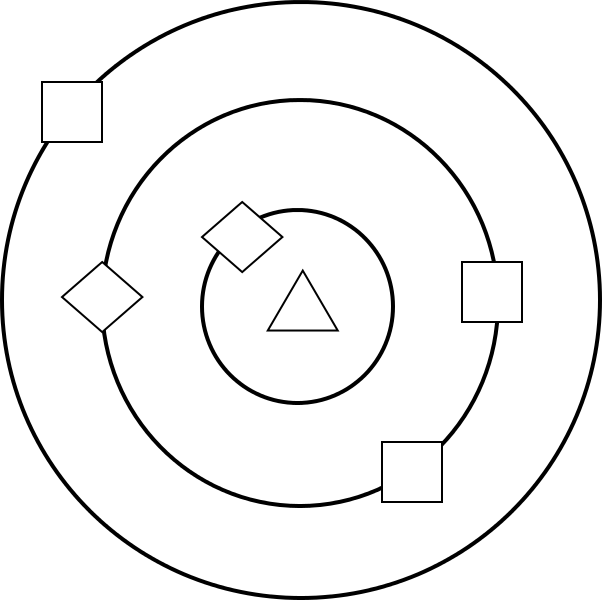
\includegraphics[width=0.5\textwidth]{figures/knn.png}
}
\subfloat[\textsc{KNN} com credibilidade]{
    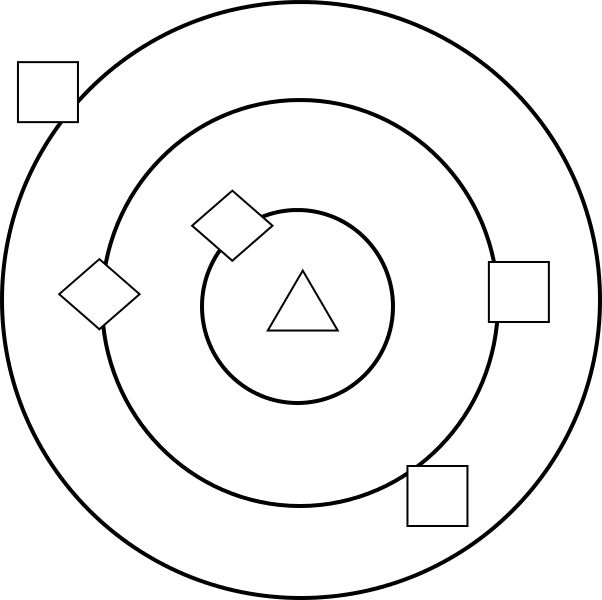
\includegraphics[width=0.5\textwidth]{figures/knncred.png}
}
\caption{Em (a) temos o algoritmo original dos $K$ vizinhos mais próximos e em (b) temos um possível resultado da utilização da credibilidade conjuntamente ao \textsc{KNN}.  
\label{fig::KNNantesedepois}}
\end{figure}

Levando em consideração o que foi mostrado até esse ponto, sendo $X_1$ a instância de teste, $X_2$ a de treino e $c_{X_2}$ a classe a qual nossa instância de treino pertence, modificamos a Equação~\ref{eqn::distancia_cat} para:

\begin{equation} \label{eqn::distancia_cat_cred}
   dist(X_1, X_2) = \sum_{1 < i < D\ \wedge \ x_{i1} \neq x_{i2}} 1.0 + \frac{1.0}{1.0 + Cr_{cont}(x_{i1}, c_{X_2} ))}
\end{equation}

Para garantirmos o efeito mostrado na Figura \ref{fig::KNNantesedepois}, adicionamos um termo relacionado a credibilidade na Equação~\ref{eqn::distancia_cat}, um fator inversamente proporcional ao valor calculado para a credibilidade. Note que como definimos a credibilidade como sendo sempre um valor positivo, teremos que a distância entre $X_1$ e $X_2$ é sempre maior que uma unidade, sendo que maior ela será quando menor for a credibilidade. Caso não somarmos o primeiro termo 1.0 na equação acima, então teríamos valores entre zero e um para a distância, onde maiores valores para a credibilidade estariam mapeados para distâncias próximas a zero e valores baixos para distâncias próximas a um. Ambos métodos são perfeitamente compatíveis, porém para ilustrar o que foi definido e modelado na Figura~\ref{fig::KNNantesedepois} é necessário somar o fator 1.0. 


\subsubsection{\textsc{KNN} Textual.}
\label{subsubsec::knntexto}

Assim como feito na incorporação da credibilidade nos atributos categóricos, utilizamos a informação da classe do exemplo de treino e calculamos a credibilidade de um termo em relação àquela classe. Sendo $t_i$ o termo referente ao atributo $A_i$, $x_i$ a frequência do mesmo e $w_i$ o seu peso (como já explicado, usamos a métrica \textsc{IDF}, Seção~\ref{subsubsection::idf}), temos:

\begin{equation}\label{eqn::distancia_texto_cat}
    dist(X_1, X_2) = \sum\limits_{1 < i < D}\frac{  Cr_{cont}(t_{i1}, c_{X_2}) \cdot x_{i1} \cdot w_{i1} \cdot x_{i2} \cdot w_{i2} }{ ||X'_1|| \cdot ||X_2|| }
\end{equation}

Repare que utilizamos $||X'_1||$ como a norma do vetor $X_1$, levando em conta a credibilidade em relação à classe da instância de treino $X_2$, logo teríamos que $||X'_1|| = \sqrt{ ( Cr_{cont}(x_{11}, c_{X_2}) \cdot x_{11} \cdot w_{11} )^2 + ... +  ( Cr_{cont}(x_{D1}, c_{X_2}) \cdot x_{D1} \cdot w_{D1} )^2}$.

Novamente, assim como discutido na Seção~\ref{subsubsec::nbcredatributos}, existem diversas métricas que podemos utilizar para inferirmos a credibilidade de um elemento, a fim de melhorarmos a classificação do algoritmo \textsc{KNN}. Algumas dessas métricas já foram previamente discutidas e o serão novamente ao longo desse trabalho. Entretanto, voltamos a frisar que a escolha de uma função de credibilidade é dependente ao contexto que a mesma está inserida e combinar as métricas disponíveis é uma tarefa combinacional cara e, para tanto, estamos usando Programação Genética como será discutido em detalhes no Capítulo~\ref{cap::programacao_genetica}.

\subsection{\textsc{KNN} com Credibilidade Baseada em Relacionamentos.}
\label{subsubsec::knncredgrafos}

A mesma situação exposta com detalhes na Seção~\ref{subsubsec::nbcredgrafos} retoma à cena. Modelamos a credibilidade existente no relacionamento entre um exemplo de teste e um de treino. 
%tribuída a um exemplo de teste em relação a determinada classe utilizando o relacionamento que aquela instância tem com as demais instâncias de treino, levando em consideração a classe que as mesmas pertencem.
Diferentemente da modelagem da credibilidade para o conteúdo do algoritmo \textsc{KNN}, dessa vez, podemos criar apenas um modelo que se adapta a qualquer tipo de atributo, numérico, categórico ou textual. Logo, sendo $X_1$ a instância de teste, $X_2$ a instância de treino e $\alpha$ o fator somado a credibilidade de relacionamento para evitarmos valores nulos no denominador, temos:

\begin{equation}\label{eqn::distancia_grafos}
%    dist(X_1, X_2) = dist(X_1, X_2) \cdot (\alpha + Cr_{rel}(X_1, class_{X_2})) 
    dist(X_1, X_2) = \frac{ dist(X_1, X_2) } { \alpha + Cr_{rel}(X_1, class_{X_2}) }
\end{equation}

Note que estamos modificando o valor da distância calculado entre a instância de teste e a de treino, baseando no fato que quanto maior a credibilidade do relacionamento do teste $X_1$ a uma classe $c_i$, menor será a distância entre o exemplo $X_1$ e os outros exemplos do treinamento que pertencem a classe $c_i$.

Mais uma vez, podemos utilizar as várias propriedades dos grafos para calcularmos a credibilidade dos relacionamentos. Na Seção~\ref{sec::pg_cred_baseada_grafos}, definimos várias métricas que calculam essas propriedades. Por fim, usamos a Programação Genética para combinarmos essas métricas a fim de obtermos uma melhor função de credibilidade que explore o melhor possível o relacionamento exemplo-classe.

